\documentclass{amsart}
\usepackage{amssymb, amsmath, graphicx, caption, enumerate}
\graphicspath{ {images/} }
\usepackage{amsthm}
\usepackage{xargs}
\usepackage{scalerel}


\newcommand{\N}{\mathbb{N}}
\newcommand{\Z}{\mathbb{Z}}
\newcommand{\R}{\mathbb{R}}
\newcommand{\K}{\mathbb{K}}
\newcommand{\C}{\mathbb{C}}
\newcommand{\ds}{\displaystyle}
\newcommand{\op}[1]{\left(#1\right)}
\newcommand{\cp}[1]{\left[#1\right]}
\newcommand{\av}[1]{\left| #1\right|}
\newcommand{\st}[1]{\left\{#1\right\}}


\usepackage[colorinlistoftodos,prependcaption,textsize=tiny]{todonotes}
\newcommandx{\question}[2][1=]{\todo[linecolor=red,backgroundcolor=red!25,bordercolor=red,#1]{#2}}
\newcommandx{\change}[2][1=]{\todo[linecolor=blue,backgroundcolor=blue!25,bordercolor=blue,#1]{#2}}
\newcommandx{\add}[2][1=]{\todo[linecolor=OliveGreen,backgroundcolor=OliveGreen!25,bordercolor=OliveGreen,#1]{#2}}
\newcommandx{\improve}[2][1=]{\todo[linecolor=Plum,backgroundcolor=Plum!25,bordercolor=Plum,#1]{#2}}
\newcommandx{\thiswillnotshow}[2][1=]{\todo[disable,#1]{#2}}
\newcommandx{\remove}[2][1=]{\todo[linecolor=yelllow,backgroundcolor=yellow!10,bordercolor=red,#1]{#2}}


\newcommand\reallywidehat[1]{\arraycolsep=0pt\relax%
\begin{array}{c}
\stretchto{
  \scaleto{
    \scalerel*[\widthof{\ensuremath{#1}}]{\kern-.5pt\bigwedge\kern-.5pt}
    {\rule[-\textheight/2]{1ex}{\textheight}} %WIDTH-LIMITED BIG WEDGE
  }{\textheight} % 
}{0.5ex}\\           % THIS SQUEEZES THE WEDGE TO 0.5ex HEIGHT
#1\\                 % THIS STACKS THE WEDGE ATOP THE ARGUMENT
\rule{-1ex}{0ex}
\end{array}
}

\setlength{\textwidth}{\paperwidth}
\addtolength{\textwidth}{-3in}
\calclayout

\setcounter{secnumdepth}{0}
\usepackage{titlesec}
\titleformat{\section}{\center\large\bfseries}
\titleformat{\subsection}{\center}


% TOC
\setcounter{tocdepth}{1}


\begin{document}





\begin{abstract}

Obtaining the solution to stochastic inverse problems is an important challenge in computational science. By solving a stochastic inverse problem, one may find an updated  characterization of parameter space that combines  prior beliefs and observable data. Using a new approach detailed in [Butler], we may solve for a probability distribution in parameter space, $\Lambda$, such that its push-forward (\emph{i.e.,} image) through the parameter-to-data map $f$ matches the observed probability density on the data, $\mathcal{D}$. Under certain conditions [Butler, Tarantola], an approximate solution of the stochastic inverse problem can be obtained as the solution of a regularized, convex minimization problem.
  
In this proposal, we consider a noisy map $f$ from a high-dimensional $\Lambda$ to $\mathcal{D}$ of specified dimension, where the gradient of $f$ exists, but may be inaccessible. If the gradient of $f$ is accessible, the minimization problem can be solved using gradient-based descent methods. If the gradient of $f$ is inaccessible, one may apply Derivative-Free Optimization (DFO) schemes as in [Chen and Wild]. In either case,  the effectiveness of the optimization algorithm may be enhanced by performing dimension reduction in $\Lambda$ as in [Russi, Constantine]. We consider different strategies for computing the active subspace of $f(\Lambda)$ in the context of both approaches, and apply them to the data-consistent inversion of two model problems. Both of these model problems are related to stochastic inverse problems arising in the simulation of plasmas in fusion reactors.
 

\end{abstract}


\title{Thesis Proposal}

\author{Jordan R. Hall}

\maketitle



\tableofcontents

\setcounter{tocdepth}{0}




\newpage

\section{Literature Review and Framework}

In the proceeding section we provide a literature review of inverse problem theory, derivative-free (DF) optimization, and dimension reduction. In the process, we will build a theoretical framework upon which to pose research questions, state initial results, and form a research plan. 

We begin our discussion by defining a parameter space $\Lambda$ of dimension $N$, a map or ``model" $f$, and a data space $\mathcal{D}$. We assume that $\mathcal{D}$ has dimension $M$, typically with $M\leq N$. Points in $\mathcal{D}$ may be known values of $f(\lambda), \lambda\in \Lambda$; as such, we may write $d=f(\lambda)$ to denote the particular datum corresponding to the evaluation of a point $\lambda \in \Lambda$ under $f$. Points in $\mathcal{D}$ may also be \textit{observed} data, denoted $d_{\text{obs}}$, where the corresponding $\lambda\in \Lambda$ may be unknown. We allow for realizations of $f$ to be  noisy. Hence, we may model draws of $f$ with $f(\lambda)=f(\lambda)+\epsilon$, which is an additive noise structure, or $f(\lambda)=f(\lambda)(1+\epsilon)$, which is a multiplicative noise structure.


\subsection{Data-Consistent Inversion}


We follow [B,T,S] to formulate an inverse problem in our setting. Then, we briefly present the data-consistent solution; we refer to [B] for details.

\change{Avoid "so-called", if you are defining terms use em or bf and not quotes}
First, we assume we have prior knowledge of the parameter space, given by the %so-called 
 prior distribution, $\pi_\Lambda^\text{prior}(\lambda)$. In practical applications, a prior distribution may be given by application experts, but may also reflect the state of knowledge on $\Lambda$ obtained by other mathematical or statistical processes. Second, we assume that we have a so-called ``observed" density, $\pi_\mathcal{D}(d)$, which represents our uncertain state of knowledge of observed data and is uncertain due to noise in $f$ and potential measurement error. Informally, the inverse problem is the task of finding an \textit{updated} probability distribution, $\pi_\Lambda^\text{update}$, in $\Lambda$ space that combines the given prior information and data.

It has been shown [] that the so-called classical Bayesian or statistical Bayesian [T,S] solution to the inverse problem is not generally a ``pull-back probability measure," in the sense that the image of the updated distribution $\pi_\Lambda^\text{update}$ under the map $f$, called the push-forward, is not equal to (and often not ``close" to) the ``observed" probability distribution, $\pi_\mathcal{D}$. 



\change{Define the forward uncertainty problem.  i.e. given distributions on $\lambda \in \Lambda$, solve for the pdf of $f(\lambda)$.  The forward uncertainty problem is different from 
forward model or the forward map, which is simply evaluating $f(\lambda)$.}

Data-consistent inversion (DCI) seeks an updated solution $\pi_\Lambda^\text{update}$ for which the push-forward exactly equals $\pi_\mathcal{D}$. To obtain such a solution, it is necessary to compute the push-forward of $\pi_\Lambda^\text{prior}$. We may form the push-forward of the prior by solving a \textit{forward problem}; with certain assumptions on $f, \Lambda,$ and $\mathcal{D}$ the forward problem may be straightforward, with other assumptions, this problem is non-trivial. We denote the solution to the forward problem with $\pi_\mathcal{D}^{f(\Lambda)}$. Then, as in [], the \textit{data-consistent} solution to the inverse problem is

\begin{equation} \label{eq:1}
\pi_\Lambda^\text{update}=\pi_\Lambda^\text{prior}(\lambda)\frac{\pi_\mathcal{D}(f(\lambda))}{\pi_\mathcal{D}^{f(\Lambda)}(f(\lambda))}.
\end{equation}

\subsection{Optimization Methods for Solving Inverse Problems}

With our assumptions of an expensive $f$ and a high-dimensional $\Lambda$, approximately solving the forward problem to obtain the push-forward density generally requires some type of kernel density estimation (KDE), which converges slowly, typically at Monte Carlo rates of $ \frac{1}{\sqrt{N}}$. As in [Tarantola], depending on $f$, the solution to the inverse problem can be obtained exactly or approximately by solving an equivalent deterministic convex optimization problem. As in [Butler], we may alter the aforementioned classical formulation of the deterministic optimization problem to ensure we obtain, depending on $f$, the \textit{data-consistent} (exact or approximate) solution to the inverse problem.

We begin by examining the classical formulation of a deterministic optimization problem which corresponds to either exactly or approximately solving the stochastic inverse problem (SIP) under consideration. In particular, for a linear map $f$, the exact solution is obtained; for nonlinear maps, we obtain an approximate solution. As in [Taratola], given observed data $d_{\text{obs}} \sim \pi_\mathcal{D}$ and a draw $\lambda_\text{prior}\sim \pi_\Lambda^\text{prior}$, we define a \textit{misfit function}

\begin{equation} \label{eq:2}
S(\lambda)=\frac{1}{2}\left(||f(\lambda)-d_{\text{obs}}||_\mathcal{D}^2+||\lambda-\lambda_{\text{prior}}||_\Lambda^2\right).
\end{equation}

The misfit function appears in the classical (i.e., statistical Bayesian) solution to the inverse problem, as $\pi_\Lambda^\text{update}(\lambda) \sim \exp(-S(\lambda)).$ We observe, as in [T], that finding the MAP point is equivalent to finding the $\lambda$ for which $S$ is minimized.

As in the preceding section, we assume $\pi_\Lambda^\text{prior}$ is a known probability density with mean $\bar{\lambda}$ and covariance matrix $C_\Lambda$; likewise, $\pi_\mathcal{D}$ is a known probability density with mean $\bar{d}$ and covariance matrix $C_\mathcal{D}$. As in [B], we can use the assumed covariance structures on $\Lambda$ and $\mathcal{D}$ to rewrite \eqref{eq:2} as


\begin{equation} \label{eq:3}
S(\lambda)=\frac{1}{2}\left(\left|\left|C_\mathcal{D}^{-1/2}(f(\lambda)-d_{\text{obs}})\right|\right|_2^2+\left|\left|C_\Lambda^{-1/2}(\lambda-\lambda_{\text{prior}})\right|\right|_2^2\right).
\end{equation} 

Classically ([T]), it is assumed that $\pi_\Lambda^\text{prior}$ and $\pi_\mathcal{D}$ are Gaussians, and the misfit function is specified by $\lambda_{\text{prior}}=\bar{\lambda}$ and $d_{\text{obs}}=\bar{d}$ in our notations. In \eqref{eq:2} and \eqref{eq:3}, we choose to define a more general misfit function, so that we may consider the ``misfit" given any draws $\lambda_{\text{prior}}\sim \pi_\Lambda^\text{prior}$ and $d_\text{obs} \sim \pi_\mathcal{D}$. The misfit function defined above can be understood term-by-term. Given $\lambda \in \Lambda$, the term $||f(\lambda)-d_{\text{obs}}||_\mathcal{D}^2$ corresponds to finding the mismatch between the observed $d_\text{obs}$ and $f(\lambda)$ in data space; the term $||\lambda-\lambda_{\text{prior}}||_\Lambda^2$ corresponds to performing Tikhonov regularization, which improves conditioning in minimizing $S$ over $\Lambda$. The minimum of $S$ is typically referred to as the maximum a posteriori point or \textit{MAP point}.

Authors in [] rewrite $S$ so that a data-consistent MAP point may be obtained. An additional ``deregularization" term is appended so that if a unique solution exists, the regularization will be ``turned off." For now, we assume that $f$ is linear (or can be linearized locally [T]), and write the matrix $A$ to define that action of $f$ on $\Lambda$. We also assume that $\pi_\Lambda$ and $\pi_\mathcal{D}$ are Gaussian. In this case, we write the \textit{data-consistent misfit function,}




\begin{equation} \label{eq:4}
T(\lambda)=\frac{1}{2}\left(\left|\left|C_\mathcal{D}^{-1/2}(f(\lambda)-d_{\text{obs}})\right|\right|_2^2+\left|\left|C_\Lambda^{-1/2}(\lambda-\lambda_{\text{prior}})\right|\right|_2^2-\left|\left|C_A^{-1/2}(f(\lambda)-f(\lambda_{\text{prior}}))\right|\right|_2^2\right),
\end{equation} 

\noindent where $C_A=AC_\Lambda A^T$. We note that in the case that $\pi_\Lambda$ and $\pi_\mathcal{D}$ are Gaussian and $f$ is linear, the data-consistent solution to our inverse problem is given exactly by $\pi_\Lambda^\text{update}(\lambda)\sim \exp(-T(\lambda))$. Generally, the deregularization term will ensure a solution that updates the distribution on $\Lambda$ only in the directions in which the data is informative. The linear case illustrates the action of the un-regularization term. In the case that a unique solution to the inverse problem exists for a linear $f$ (i.e., $N=M$ and $A$ is full rank), the un-regularization term will equal the Tikhonov regularization term, so that the MAP point solves the data misfit exactly. When the problem is under-determined ($N>M$), then with a linear $f$, the data-consistent solution to inverse problem will lie in a hyperplane in $\Lambda$ containing all the possible points that could have produced the $M$ observed data. Regardless of whether $N=M$ or $N>M$, the MAP point obtained by minimizing the ``classical" misfit, in general, will not be a point that could have produced the observed data. We highlight the difference in solutions in the example below.

\vspace{.125cm} 

\noindent \textbf{Example 1.} \textit{Let $f(\lambda)=2\lambda$, $\lambda_\text{prior}=0.1$, $C_\Lambda=[0.5],$ $d_\text{obs}=0.25$, and $C_\mathcal{D}=[0.25]$; note, $N=M=1$. Then we find that $S(\lambda)=2((2\lambda-0.25)^2+(\lambda-0.1)^2)$, which is minimized by $\lambda^*_S=3/25$. Assuming that $\lambda_\text{prior}$ and $d_\text{obs}$ are the means of Gaussians with standard deviations corresponding to the above covariance matrices, we have $\pi_\Lambda^\text{post} \sim \exp(-S(\lambda_S^*))$. Notice $f(\lambda^*_S)=6/25\neq d_\text{obs}$. We write $T(\lambda)=2(2\lambda-0.25)^2$, which is minimized by $\lambda^*_T=1/8$. Notice $f(\lambda^*_T)=d_\text{obs}$. With Gaussian assumptions on the prior and data, we have $\pi_\Lambda^\text{post} \sim \exp(-T(\lambda_T^*))$.}



\vspace{.125cm}

In the preceding example, we observe for linear $f$ and $N=M$, the classical MAP point, given by $\lambda_S^*=0.12$ and obtained by minimizing $S$, strikes a balance between the prior belief that $\lambda=0.1$ and the fact that the value $\lambda=0.125$ is the pre-image of $0.25$ under $f$, the observed data point. The data-consistent MAP point, given by $\lambda_T^*=0.125$, is exactly the pre-image of $d_\text{obs}$. Indeed, since the linear map $A$ is full rank in Example 1, the third term in \eqref{eq:3} fully deregularizes (cancels out) the second term, so that the minimum of $T$ is actually just the minimum of the first term, the data mismatch. We see here that classical Bayesian inverse problem theory and DCI ask and answer different questions. For a similar, concrete example where the number of parameters $N$ is greater than the number of data, $M$ (so that the problem is under-determined), we refer the interested reader to []. 
\question{See below, you can use Tim's example}


So far, we have presented a deregularization term in \eqref{eq:3} which will hold only for linear (or linearizable) $f$ and Gaussian assumptions on the parameter and data spaces. For general nonlinear functions $f$, the deregularization must be rewritten. Here, we arrived at an open research question, which we discuss further in the proceeding section.



\todo{Varis: This was the best I could do, and I am not sure it is correct! Can you edit/perhaps add some content here??}

\question{I have the following figure, which corresponds to the example from Tim's talk}. 
\change{Add the 2nd example which includes deregularization, here?}

\begin{figure}
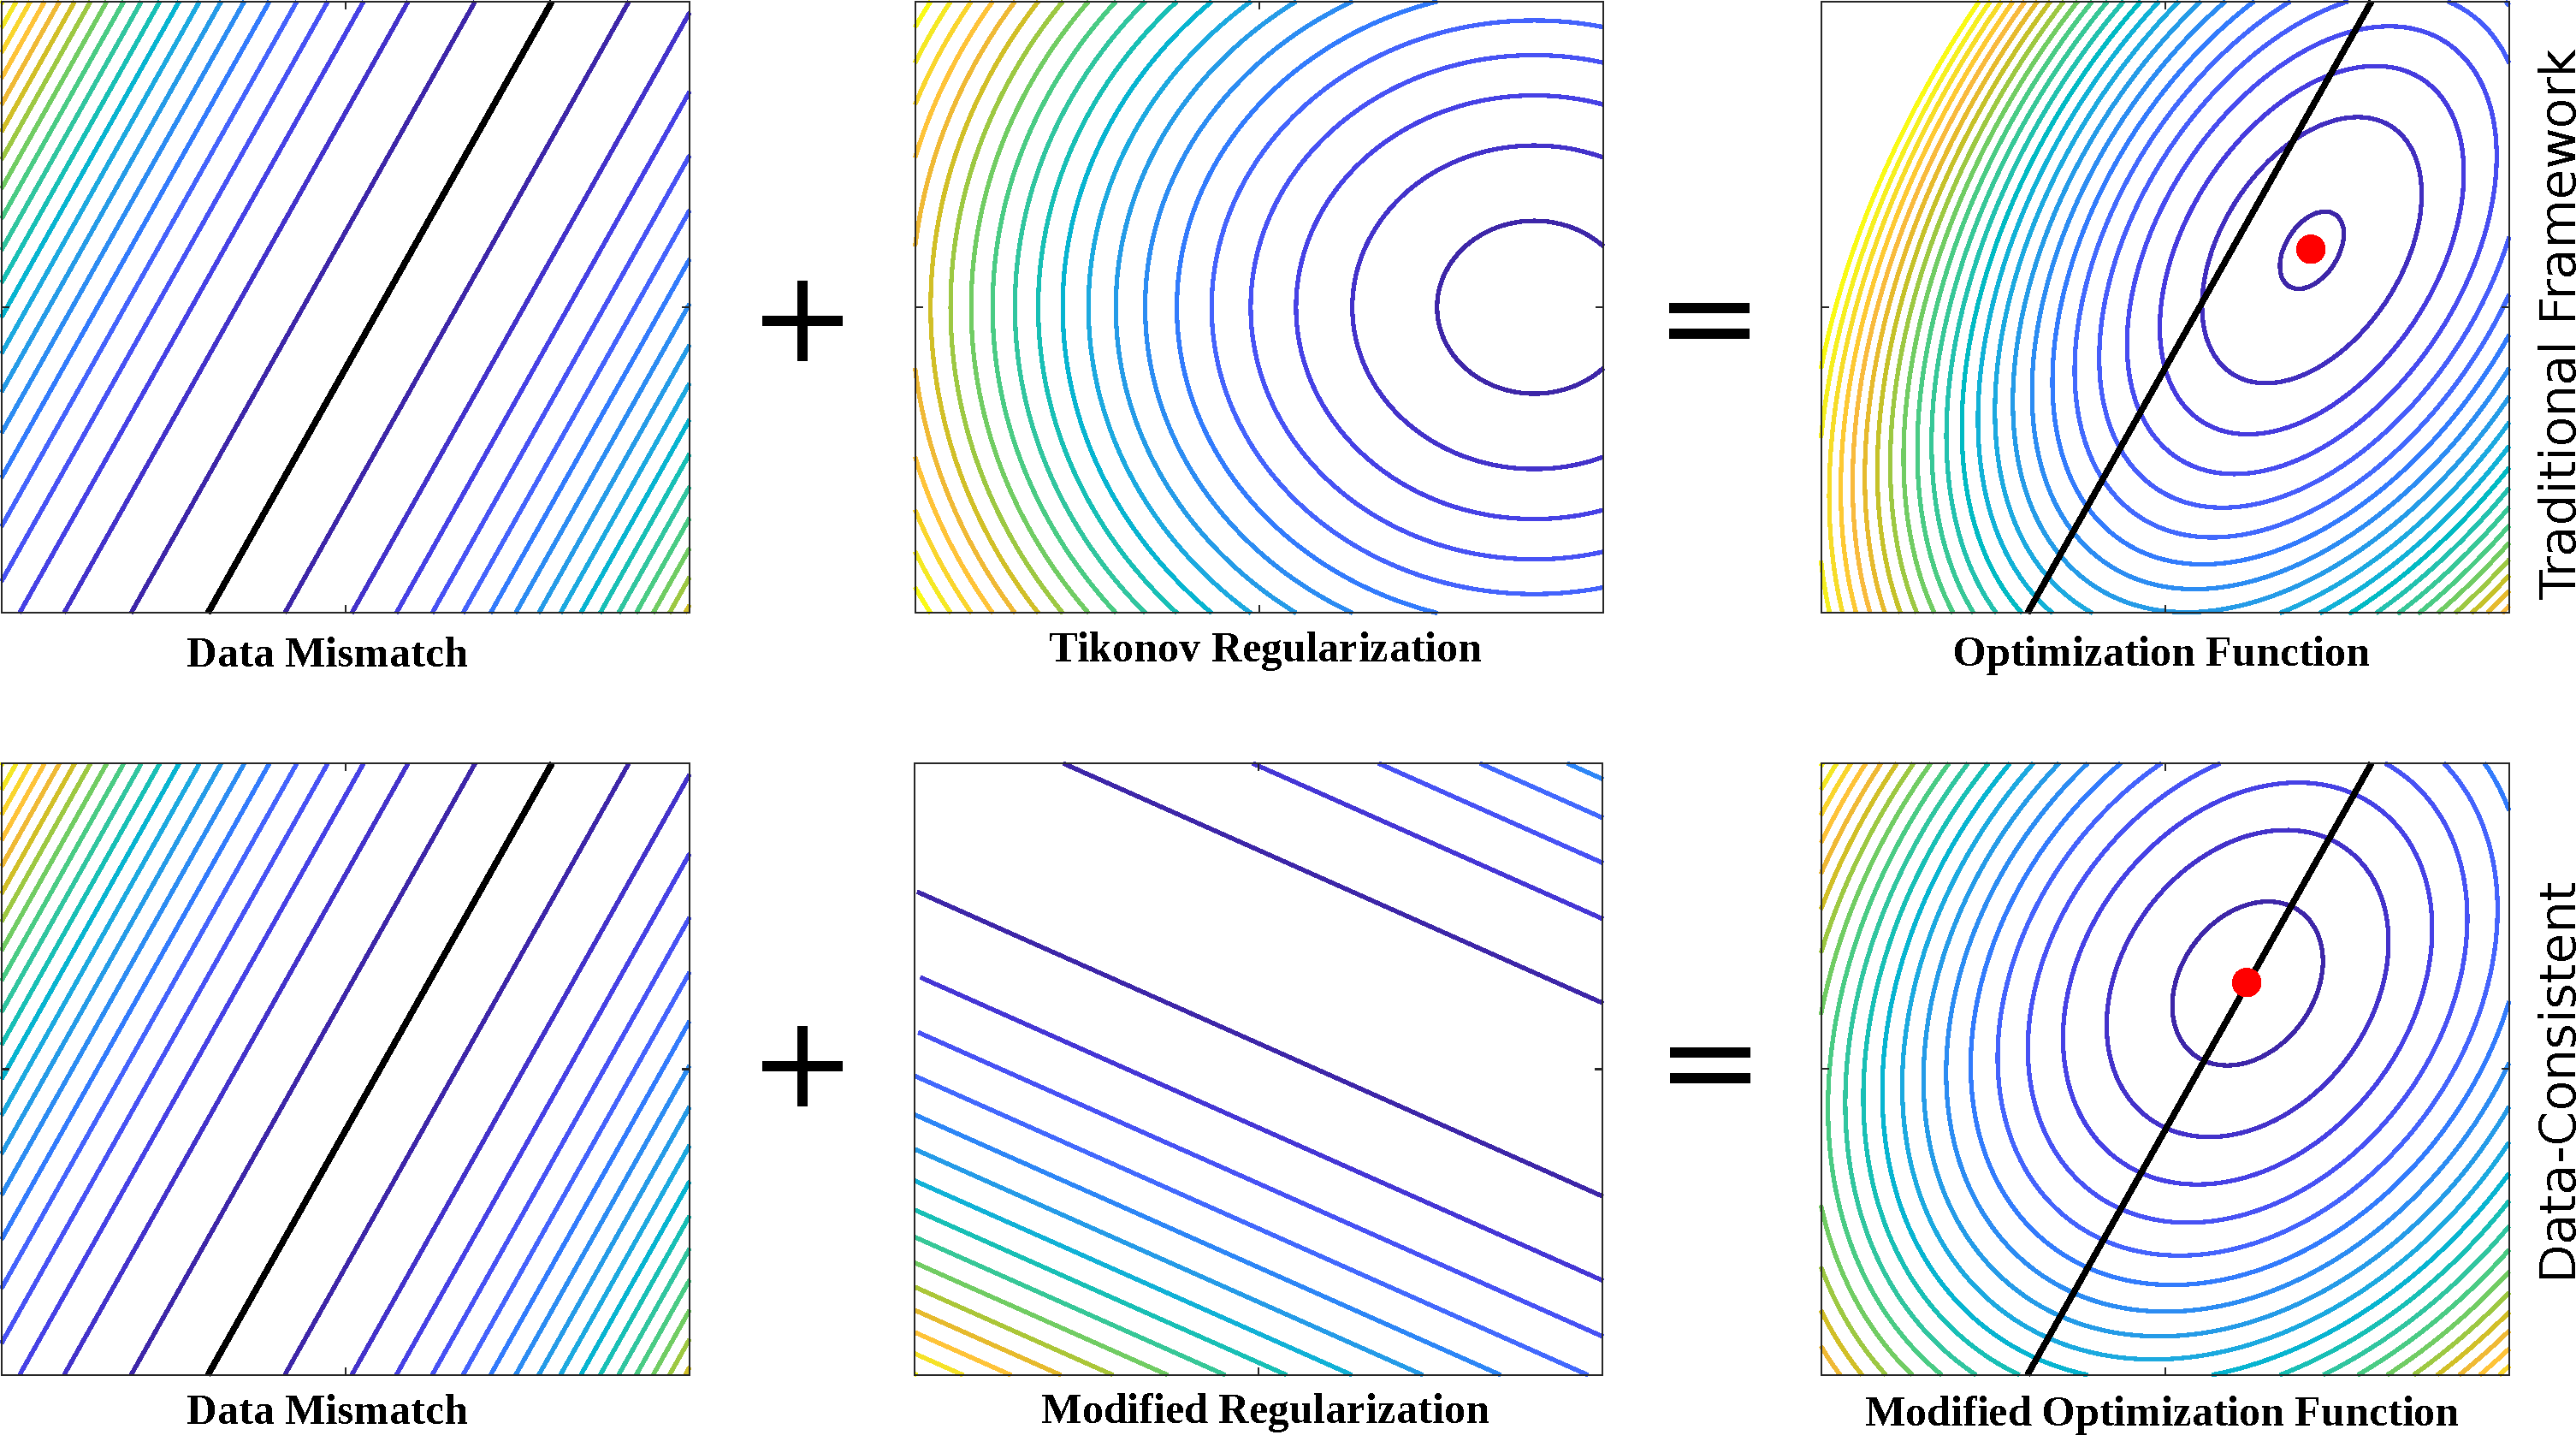
\includegraphics[width=\textwidth]{Regularization-all-in-one.pdf}
\end{figure}







\subsection{Dimension Reduction}

\question{Why? Motivate Dimension Reduction}
In our setting, it may be advantageous to perform dimension reduction on $f$. In particular, we shall consider Active Subspace methods described by Paul Constantine in [] and an equivalent method by T.M. Russi in []. These techniques seek to explain outputs $f(\Lambda)$ in a subspace $A \subset \Lambda$ for which the $\dim (A) <N$. Here we discuss the theoretical formulation of $A$, but also how it may be found in practice.

We begin by noting $\nabla f(\lambda)\in \Lambda$ is a column vector of the same dimension as inputs $\lambda$ with rows containing the $N$ partial derivatives of $f$, which for this discussion we assume exist, and are square integrable in $\Lambda$ equipped with some probability density that is positive everywhere in $\Lambda$ and 0 otherwise; for instance, we could consider $\pi_\Lambda^\text{prior}(\lambda)$, the density describing our prior state of knowledge, which we choose to abbreviate as $\pi_\Lambda$ for this discussion. In classical active subspace analysis, one transforms inputs $\lambda$ to the origin with some fixed variance, typically so that $\lambda\in [-1,1]$. Then, as in [C,E,W, and C], we may write

\begin{equation} \label{eq:6}
W=\int_\Lambda \nabla f(\lambda) \nabla f(\lambda)^\top  \pi_\Lambda(\lambda) d\lambda,
\end{equation} 

\noindent which is an $N\times N$ symmetric positive semi-definite matrix which defines a certain covariance structure of $\nabla f$ over $\Lambda$. This interpretation of \eqref{eq:5} leads one to the idea of computing the Singular Value Decomposition of $W$,

\begin{equation} \label{eq:7}
W=U\Sigma V^*,
\end{equation} 

\noindent where $U$ is $N \times N$ unitary, $\Sigma$ is $N \times N$ diagonal with the singular values of $W$ along its diagonal, and $V^*$ is $N \times N$ unitary. With the singular values of $W$ in hand, we search for a drop-off in the spectrum of $W$. In detail, we plot the singular values, $\{\sigma_i\}_{i=1}^n$ and seek a drop-off in magnitude between some pair of singular values, $\sigma_{j}$ and $\sigma_{j+1}$. The active subspace is the span of $u_1,\ldots,u_{j}$, which are the first $j$ columns of $W$, the so-called ``left singular vectors" of $W$. 

The fact that $u_1,\ldots,u_{j}$ correspond to the nontrivial singular values is exactly why they account for the most amount of variance in function values. In fact, one can view AS analysis as an artful choice of principal components after a \textit{full} Principal Component Analysis (PCA) is performed in the gradient space $W$; for more details on this viewpoint, we refer the interested reader to Section 6.4 in T.M. Russi.

For a point $\lambda \in \Lambda$, we define

\begin{equation} \label{eq:8}
  \mathcal{P}_A(\lambda)=\sum_{i=1}^{j}\left( u_i^T \lambda\right)u_i \in A, 
\end{equation}

\noindent which is a projection of the point $\lambda$ in the ``active directions" of $f$. We call this projection an ``active variable," which is a point in the active subspace $A$. We have arrived at the property that 

\begin{equation} \label{eq:9}
f\left(\mathcal{P}_A(\lambda)\right) \approx f(\lambda).
\end{equation}

In practice, finding an active subspace of $f$ will require forming an approximation to $W$ in a Monte Carlo fashion; see []. We choose to present a Monte Carlo approach that is simple to implement. In short, for a random draw $\lambda_i \in \Lambda$, we will find its evaluation under the approximate or analytic gradient (depending on whether we have $\nabla f$ analytically), and store the row vector $f(\lambda_i)^\top$ in a matrix with an SVD corresponding to \eqref{eq:6}, up to scaling.

In the following, we assume that we lack an analytic form of $\nabla f$; if the analytic gradient is available, the proceeding Monte Carlo method remains valid, and all notations corresponding to approximating $\nabla f$ may be dropped.

\question{Maybe switch $M$ to $S$ for samples?  As $M$ was the dimension of the data space above}

One initializes the method by performing $M$ random draws of $\lambda_i \in \Lambda$. We then compute $f(\lambda_i)$ for all $i=1,\ldots,M$ samples, which we note will require, at the very least, $M$ evaluations of $f$; in a realistic setting, this would require $M$ solves of a model (e.g., $M$ solves of a PDE constrained system). In our notations, we have $\mathcal{D}=\{f(\lambda_i)\}_{i=1}^M$. Next, we need $\nabla_\Lambda f$ evaluated at $\lambda_i$ for all $i=1,\ldots,M$, which we assume that we do not have in closed analytic form. Hence, we generally need some gradient approximation method, and typically a locally linear approximation to the gradient is a fair balance between reasonably estimating the gradient and not pushing computational expenses to an unreasonable regime. With this approximation formed, we denote each estimation to $\nabla f(\lambda_i)$ with $\reallywidehat{\nabla f}(\lambda_i)$ and we define the $N \times M$ matrix

\begin{equation} \label{eq:10}
\tilde{W}:=\begin{bmatrix}
\reallywidehat{\nabla f}(\lambda_1)^\top
\cdot \cdot \cdot
\reallywidehat{\nabla f}(\lambda_M)^\top\\
\end{bmatrix}.
\end{equation}  

Forming the SVD of $\tilde{W}$, $\tilde{W}=\tilde{U}\tilde{\Sigma}\tilde{V}^*$, we search for a drop off in the magnitude of the singular values $\{\tilde{\sigma}_i\}_{i=1}^M$. Assuming such a drop off occurs for an index $j:1<j<M$, we have the $j$ corresponding left singular vectors,$ \tilde{u},\ldots,\tilde{u}_{j}$.  We let $A\left(f;\mathcal{D}\right):=\text{span}\{\tilde{u},\ldots,\tilde{u}_{j}\}$ to denote the active subspace of $f$ with respect to the data $\mathcal{D}$. We choose to use a notation with $\mathcal{D}$ included to emphasize the dependence of the active subspace on the random draws made in $\Lambda$, which led to our particular $\mathcal{D}$.

In practice, we can check the extent to which the active subspace accounts for functions values $f(\lambda)$ 
by checking for resolution in a so-called ``sufficient summary plot" [Constantine], where we plot active variables against function values. In these plots, we hope to see a pattern between the active variables versus the actual function values. For example, if $f$ is quadratic in its active variables, then we expect to see quadratically-resolved sufficient summary plots. We will revisit sufficient summary plots in the proceeding sections. For now, we continue our discussion with the understanding that sufficient summary plots allow us to check the ``fit" of the active subspace.





\subsection{Derivative-Free Optimization}

%\todo{Varis: I'll write an intro here connecting DF algorithms to noisy simulations due to turbulence/chaos to }
Many important physical systems possess turbulent or chaotic behavior.  The physical state of the system $u(x,\lambda)$ and the corrsponding parameter
to observable map $f(u(x,\lambda))$ may be modelled as a stochastic process, or as a deterministic function with additive or multiplicative ``noise''.  
In this setting, the efficient extraction of accurate gradients of $f$ in parameter space is a challenging undertaking, as popular techniques based on
linearization, including adjoint methods, are inaccurate\cite{QiQi}.  The finite-difference approximations to $\nabla f_\Lambda$ 
involve $N=\text{dim}\Lambda$ 
additional, usually nonlinear model solves for the physical system state $u(x,\lambda_i + \delta \lambda_i)$, and is greatly polluted by the noise in $f$.

As a consequence of these difficulties, the approximate data-consistent solution of a SIP in this setting by optimization techniques will need algorithms
that do not require gradient information from $f$.  
We consider derivative-free optimization (DFO) algorithms suited for additive and multiplicative noise as in [C/W]. This technique requires nothing more than evaluations of the noisy model and random draws from a normal distribution. Briefly, this method finds a new iterate by randomly perturbing the previous iterate in $\Lambda$; iterates are not allowed to stray much, though, due to relatively small smoothing factors and step sizes. The smoothing factor and step size in the DF algorithms are of great importance to their convergence and termination. As in [Chen and Wild], both the smoothing factor and step size will depend on a scale factor of the $L_1$ Lipschitz constant of $f$. As such, it will be of interest to obtain estimates of $L_1$, which is not straightforward in a gradient-free setting. We refer to [Others] for Lipschitz constant learning in this setting, and discuss this problem more thoroughly in the proceeding sections.


\question{The reference here is Nesterov?}
In detail, as in [], we consider the problem

\begin{eqnarray} \label{eq:11}
\min_{x\in\R^N} \quad \mathbb{E}\left[f(x)+\nu (x; \xi))\right],
\end{eqnarray} 

\noindent where the authors assume that:

\begin{enumerate}[(i.)]

\item $f: \R^N \to \R$ is convex;

\item $\xi \in \Xi$ is a random variable with probability density $P(\xi)$;

\item for all $x \in \R^N$ the additive noise model $\nu$ is independent and identically distributed, has bounded variance $\sigma_a^2$, and is unbiased; i.e., $\mathbb{E}_\xi (\nu(x;\xi))=0$.



\end{enumerate}

The use of the $\mathbb{E}(\cdot)$ expected value notation is a mathematically precise way of expressing the fact that the authors view function evaluations as a random draw, in the sense that true function values $f(x)$ are perturbed by a random vector in an additive or multiplicative fashion. Indeed, others [] make similar assumptions, viewing evaluations of $f$ as a black-box process with noise, which obscures the true value of draws $f(\lambda)$.

Chen and Wild propose the ``STARS (STep-size Approximation in Randomized Search)" algorithm, which: uses small perturbations in the domain $\Lambda$ given by the addition of a random vector with components drawn from a normal distribution; computes the function value at the randomly perturbed point with additive or multiplicative noise drawn from a specified distribution; and updates iterates using a Gaussian-smoothed finite-difference scheme for approximate gradient information in a gradient descent scheme. We will examine the STARS algorithm in closer detail in the following sections. For now, we point out that the algorithm requires the ability to evaluate the model, and needs access to random draws from a normal distribution and the distribution from which noise is drawn. All in all, the algorithm can be implemented in about 10 lines of code in \texttt{python}.





\section{Research Questions}

In the following section, we pose research questions to be investigated within the framework provided in the preceding section. 

\subsection{Impact of Noise on MAP Point and Updated Prior}

\subsection{Learning and Sampling}

\subsubsection{Learning the Active Subspace}

\subsection{Using the Active Subspace} Generally, if an active subspace $A$ exists for a model $f$, dimension reduction may be performed by, for instance, projecting inputs $\lambda$ into $A$ then evaluating $f$ for the projection; i.e., form $f\left(\mathcal{P}_A(\lambda)\right)$. Computational expense may be saved by projecting points $\lambda$ into their so-called active variables, since such projections are of lower dimension than $\lambda$. This property gives the ability to save computational expense for a number of problems in Uncertainty Quantification, including optimization, representation and solving inverse problems. In the following, we consider ways in which we may use the information given by an active subspace $A(f;\mathcal{D})$.

\subsubsection{DFO in the Active Variables Only} Given some $f$ and its corresponding active subspace $A(f;\mathcal{D})$ found by the Monte Carlo method discussed in the preceding section, we are interested in investigating the effectiveness of only optimizing $f$ in its active variables. There are several approaches one may consider, and handful of those approaches and their corresponding results are discussed in the proceeding section. The most compelling approach we have observed is to modify the DFO algorithm discussed above to only take random walks in directions lying in $A$. That is, at iteration $k$, standard DFO algorithms [CW] use random walks given by drawing a random vector $v^{(k)}$ of dimension $N$ in which every component $v_i^{(k)},i=1,\ldots,N$ of $v$ is  drawn from a specified normal distribution. Instead, given the first $j$ singular unit vectors $u_1,\ldots,u_j$ corresponding to the SVD of $\hat{W}$, one may take $j$ draws from a specified normal distribution, which we denote with $s_i\sim N(\mu,\sigma^2)$, and form the random vector $v$ for the $k$-th step in a DFO algorithm as $v^{(k)}=\sum_{i=1}^js_iu_i$, which is just a linear combination of the active variables of $f$ with coefficients given by random draws; we see that such a vector could be interpreted as a random walk in $A$.

Relevant research directions include: considering other ways to embed the information from $A$ within a DFO scheme; analyzing the difference between minimizing $f$ in all its variables versus only in its active subspace; considering ways in which the problem may be solved with the mentioned techniques in tandem, such as using a ``burn-in" phase in which $f$ is minimized over all of $\Lambda$ followed by an active variables minimization.


\subsubsection{Representations and Surrogate Modeling} We are generally interested in the representation and surrogates one may form with an active subspace. If $f$ is truly a black box, then it lacks an analytic form we can access. By performing dimension reduction, it is possible to test the resolution of function values $f$ versus active variables by forming a sufficient summary plot or ``response surface" []. Depending on the quality and form of the resolution, one may (or may not) be able to discern the relation between $f$ and its active variables visually, by fitting a surrogate through the response surface and testing the fit, or both. Representing $f$ with a lower-dimensional surrogate may help with solving other problems of interest. In particular, we may be able to solve a forward problem at lower cost, or pose the convex optimization for solving an inverse problem with such a representation used to form the misfit functions considered in the preceding section.


\subsubsection{Solving the Forward Problem} If the action of the map $f$ can be captured by a lower-dimensional representation, we may be able to more cheaply solve for the push-forward needed for DCI. Research directions include: generally comparing the cost of solving the forward problem with KDE for an $f$ defined in its full variables versus some surrogate for $f$ defined over $A$; analyzing differences in MAP points and updated densities in $\Lambda$ when the push-forward is obtained from its full variables or only from active variables.

\subsubsection{Forming the Misfit Function} Again, if $f$ can be represented in a lower dimension than that of $\Lambda$, then it may be possible to form the misfit functions with a surrogate for $f$.

\subsection{Application: Callibrated Anomolous Diffusion in Tokamak Plasmas}
\todo{Varis: I'll write this, detailing the target application}

\subsection{Application: Magnetic Equilibria in Tokamaks}
\todo{Varis: I'll write this, covering Grad-Shafonov Equations, and why these MHD equilibria are important to kinetic simulations.}


\section{Preliminary Results and Research Plan}



\todo{Varis: I'll write a brief section transitioning from current toy problems to pde models to plasma physics models}



\section{Timeline}


%%%%%%%%%%%%%% References %%%%%%%%%%%%%%%%%%%%%%%%%



%\bibitem{Constantine} Constantine, Paul G. ``Active Subspaces: Emerging Ideas for Dimension Reduction in Parameter Studies." SIAM, 2015. 


%The Active Subspaces software library and interactive Jupyter notebooks can be found at \texttt{https://github.com/paulcon/active\_subspaces}.

%\bibitem{Chen and Wild} Chen and Wild. ``Randomized Derivative-Free Optimization of Noisy Convex Functions." Funded by the Department of Energy. 2015.

%\bibitem{Russi} Russi, Trent M. ``Uncertainty Quantification with Experimental Data and Complex System Models." Dissertation, University of California Berkeley. 2010.

%bibitem{Smith}  Smith, Ralph.``Uncertainty Quantification: Theory, Implementation, and Applications.” SIAM, 2013.

\end{document}
